\chapter{Self-Sufficient Itemset Stream Mining}
\label{chapt:ASSIM}
Our earlier chapters have introduced definitions and problems that target mining interesting association rule from unlabelled data streams where data is transactional item-based using unsupervised learning. In this chapter, we focus on how to discover self-sufficient itemsets from unlabelled data streams.

There has been some research in the area of interesting association rule mining where researchers try to capture patterns involving events that happens frequently or appear in a certain pattern in a static dataset. Although much of the research focus in using ``support-confidence'' framework on finding association rule, self-sufficient are shown to be more accurate and adaptive by using several statistical tests. Until now, most of the research on this area concentrates only on finding self-sufficient itemsets in a static dataset. With the proliferation of applications which generate data streams, such as network logs and banking transactions, applying techniques that mine from static datasets onto dynamic data streams is not practical. In this chapter, we address the research problem of mining self-sufficient itemsets from dynamic data streams and propose an adaptive approach.

The main contributions of this chapter are:
\begin{itemize}
\item We propose a novel approach called  Adaptive self-sufficient Itemset Miner (ASSIM), which facilitates discovery of self-sufficient itemsets in a data stream environment with regional drift detection.
\item With ASSIM we discuss the idea of using a sliding window to achieve actual online learning for data stream rather than batch processing.
\end{itemize}

\section{Adaptive Self-Sufficient Itemset Miner (ASSIM)}
%What does ASSIM do? 
To mine self-sufficient itemsets and to solve the regional concept drift problem at the same time, we propose a new technique: Adaptive self-sufficient Itemset Miner (ASSIM). ASSIM is able to mine self-sufficient itemsets in an online mode, and at the same time, detect regional drifts among generated self-sufficient itemsets and adapt the drifts to the self-sufficient itemset generation process.

%Why do we need ASSIM?
The current self-sufficient miner \cite{ssi} is designed for static databases. To use this technique unaltered on a data stream has its pitfalls. This includes regional concept drifts that may occur over time in data stream, making previously generated self-sufficient itemsets inaccurate. We can adapt self-sufficient miner by generating itemsets at fixed intervals but this is inefficient, and there may be a delay between when changes happen in the data stream to when the new set of itemsets are generated. Another possibility is that if the intervals are set too far apart we may miss out on generating those itemsets all together. Our framework is designed to overcome this problem.


\begin{figure}[h!]
    \centering
\tikzstyle{decision} = [diamond, draw, fill=blue!20, 
    text width=4.5em, text badly centered, node distance=3cm, inner sep=0pt]
\tikzstyle{block} = [rectangle, draw, fill=blue!20, 
    text width=8em, text centerd, rounded corners, minimum height=4em]
\tikzstyle{line} = [draw, -latex']
\tikzstyle{cloud} = [draw, ellipse,fill=red!20, node distance=5cm,
    minimum height=4em]

\resizebox {\columnwidth} {!} {
\begin{tikzpicture}[node distance = 4cm, auto]
Bass
    \node [block] (init) {Batch Size Calculator};
    \node [cloud, left of=init] (data) {$D = T_1, T_2, \ldots T_n$};
    \node[above of = data,node distance=1cm]{Input (Data Stream)};
    \node [block, right of=init] (system) {Self-sufficient Itemset Generator};
    \node [block, right of=system] (rcda) {Regional\\ Concept Drift Adaptor (RCDA)};
    \node[cloud, right of = rcda](SSI){Self-sufficient Itemsets};
    % Draw edges
    \path [line] (data.east) |-(init);
    \path [line] (init) |- (system);
    \path [line] (system) |- (rcda);
    
    \path[line, dashed] (rcda.south) -| ([xshift=0cm, yshift=-1cm]rcda.south) -- ([xshift=0cm, yshift=-1cm]system.south) |- (system.south);
    \path[line](rcda.east) |- (SSI);
\end{tikzpicture}
}
    \caption{Framework of Adaptive Self-sufficient Itemset Miner }
    \label{fig:ASSIM}
\end{figure} 


An illustration our ASSIM framework is shown in Fig. \ref{fig:ASSIM}. It gives a general idea of the structure of ASSIM and how the data flows inside ASSIM.
As transactions are fed into ASSIM, they will be processed first in the Batch Size Calculator (BSC) to get an appropriate batch size before we enter the itemset mining process. The calculation of the batch size is crucial to avoid over-fitting. We realised that there are possible minor fluctuations within a data streams. Thus, a stable bucket allows for a more representative sample to be used in the mining process.   

Using the calculated batch size, the self-sufficient Itemset Generator (SSIG) can be used to generate self-sufficient itemsets. All generated self-sufficient itemsets will be checked for potential regional concept drifts by the Regional Concept Drift Adaptor (RCDA). Once a regional drift has been detected, RCDA will check the drift type and determine whether SSIG needs to generate new self-sufficient itemsets from the drift point or not.

Our Adaptive Self-Sufficient Itemset Miner algorithm is shown in Algorithm \ref{alg:assim}, which presents the top level of the technique and how its parts interact with each other.

\begin{algorithm}[h!]
\caption{Adaptive Self-Sufficient Itemset Miner (ASSIM)} 
\label{alg:assim}
\hspace*{0.02in} {\bf Input:} 
data stream $\mathcal{D}$ of transactions $\{T_1, ..., T_n\}$, $k$\\
\hspace*{0.02in} {\bf Output:} 
\textit{result}(set of self-sufficient itemsets: $S$);
\begin{algorithmic}[1]

\While{exist($\mathcal{D}$)} 
  \State $frequentItems\leftarrow$ BSC($\mathcal{D}$)
  \State stable batches $\leftarrow$ BSC($\mathcal{D}$)
  \State $S\leftarrow$ SSIG($k$, \textit{frequentItems});
  \State RCDA($S:\{s_1, ..., s_m$\}, $\mathcal{D}$: $\{T_1, ..., T_n\}$)
  \State $S'\leftarrow$ RCDA($S, \mathcal{D}$)
  \State $S \leftarrow S + S'$
\EndWhile

\State \Return set of self-sufficient itemsets $S$
\end{algorithmic}
\end{algorithm}

\section{Batch Processing}

%What does Batch Size Calculator (BSC) do?

The Batch Size Calculator (BSC) is the first part of our ASSIM framework. It was designed to handle frequency counting and batch size calculation. It provides an approximation of items’ frequencies. The main purpose of this is to ensure that a proper stable batch size was used before we mined for self-sufficient itemsets. As with any data streams, selecting an adequate learning window is essential to ensure the quality of the results produced. If the batch size is too small, the variance of the itemsets produced may be an issue. If the batch size is too large, then there is a lag or time delay between when transactions happen to when it is mined.  

%Why do we need BSC?
Data stream mining requires a stable and comparable batch size to represent the current state. In this case, Lossy Counting \cite{lossy} has been used because of its low computational cost which improves both memory and run-time processing. As only an approximated ranking list is needed, for the expansion process we used Lossy Counting. To use Lossy counting, we divide the incoming data stream into buckets. We keep a running histogram of the unique items for each transaction in the data stream. If items appear in a transaction within a bucket size, we increment the frequency count of those items. At the end of each bucket, we decrement each of the counters by 1. At the end, the most frequently viewed items `survive'.

%How does BSC works?

\subsection{Stable Batch Size}

A data stream of items $\{x_1, x_2, x_3, \C, x_m\}^{(t)}$ are the inputs at time $t$ to BSC, whereby $m$ is the number of unique items. Their frequencies will be calculated using Lossy Counting, and generate a list of top $n$ frequent items $\{a_1, a_2, \ldots, a_n\}^{(t)}$. Meanwhile, in order to calculate a stable and comparable batch size for the self-sufficient Itemset Generator, the distribution of each frequent items $D^{(t)} = \{d_a__1,$ $d_a__2$, \ldots, $d_a__n$ $\}^{(t)}$ in each Lossy Counting bucket will be calculated and compared with the prior bucket of $D^{(t-b)}= \{d_a__1,$ $ d_a__2$, \ldots, $d_a__n$ $\}^{(t-b)}$, where $b$ is the bucket size. 

When a new bucket has been processed, we average the frequency differences of top $k$ frequent items (picked from Lossy Counting) between the current bucket and the prior one. If the average frequency difference is larger than threshold $\tau$, 
\[
\frac{1}{k}\sum d_a_k^{(t)} - \frac{1}{k}\sum d_a_k^{(t-b)} > \tau,
\]   
we report the bucket number $B$ and the first batch size will be $B \times (1/e)$ whereby $e$ is the tolerance error rate for the approximation.

Our Batch Size Calculator algorithm is shown in Algorithm \ref{alg:bsc}.

\begin{algorithm}[h!]
\caption{Batch Size Calculator (BSC)} 
\label{alg:bsc}
\hspace*{0.02in} {\bf Input:} 
data stream $\mathcal{D}$, threshold $\tau$, tolerance error rate $e$;\\
\hspace*{0.02in} {\bf Output:} 
\textit{batchSize}, \textit{result}(set of stable batches);
\begin{algorithmic}[1]

\While{exist($\mathcal{D}$)} 
  \State lossyCounting($\mathcal{D}$);
  \State \textit{frequentItems} $\{a_1,a_2,...,a_n\}\leftarrow$ result from lossyCounting;
  \State \textit{bucketSize} $b\leftarrow1/e$;
  \State $D^{(t)} = \{d_a__1,$ $d_a__2$, \ldots, $d_a__n$ $\}^{(t)}\leftarrow$ distribution of each frequent item in a bucket;
  \State compare $D^{(t-b)}$ with $D^{(t)}$;
  \If{average frequency difference $> \tau$}
      \State report the current bucket number $B$;
      \State \textit{batchSize} $\leftarrow B \times (1/e)$;
  \EndIf
\EndWhile

\State \Return set of stable batches
\end{algorithmic}
\end{algorithm}

\paragraph{An Example of BSC}

Given the dataset in Table \ref{tb:tid}, we show how stable batches  built using BSC. Table \ref{tb:fq} lists the items which have more than 30\% support in the dataset, which are used for calculating stable batches in Figure \ref{fig:bsc}. In this example, threshold $\tau$ is set to 25\%, tolerance error rate $e = 1/3$.

\begin{table}[h!]
\caption{Set of Transactions in 4 Buckets Each with Length 3}
\label{tb:tid}
\centering
 \begin{tabular}{p{4cm} p{4cm}} 
 \hline\hline
 \multicolumn{2}{c}{Transactions (tid: items)}\\
 \hline
 1: a, g h & 7: g \\ 
 %\hline
 2: a, g, h, i & 8: c, h \\
 %\hline
 3: b, c, d, f & 9: c, d, h \\
 %\hline
 4: b, d, j & 10: b, f \\
 %\hline
 5: c, f, h & 11: a, h  \\
 %\hline
 6: a, e, g, h & 12: a \\
 \hline
\end{tabular}
\end{table}

\begin{table}[h!]
\caption{Frequent Items with Frequencies}
\label{tb:fq}
\centering
 \begin{tabular}{p{4cm} p{4cm}} 
 \hline\hline
 \multicolumn{2}{c}{Frequent Items (item: frequency)}\\
 \hline
 h: 6 & g: 4\\
 %\hline
 a: 5 & c: 4\\
 \hline
\end{tabular}
\end{table}

Figure \ref{fig:bsc} illustrates the process of stable batch size calculation. It monitors the distribution differences between Lossy Counting buckets. In this example, frequency difference between Bucket 3 and Bucket 4 is 50\% which is over $\tau = 25\%$, so the number 3 will be report to divide batches. The first stable batch will have a size $3 \times 1/e = 9$.

\begin{figure}[H]
\caption{Distribution difference calculation}
\label{fig:bsc}
\centering
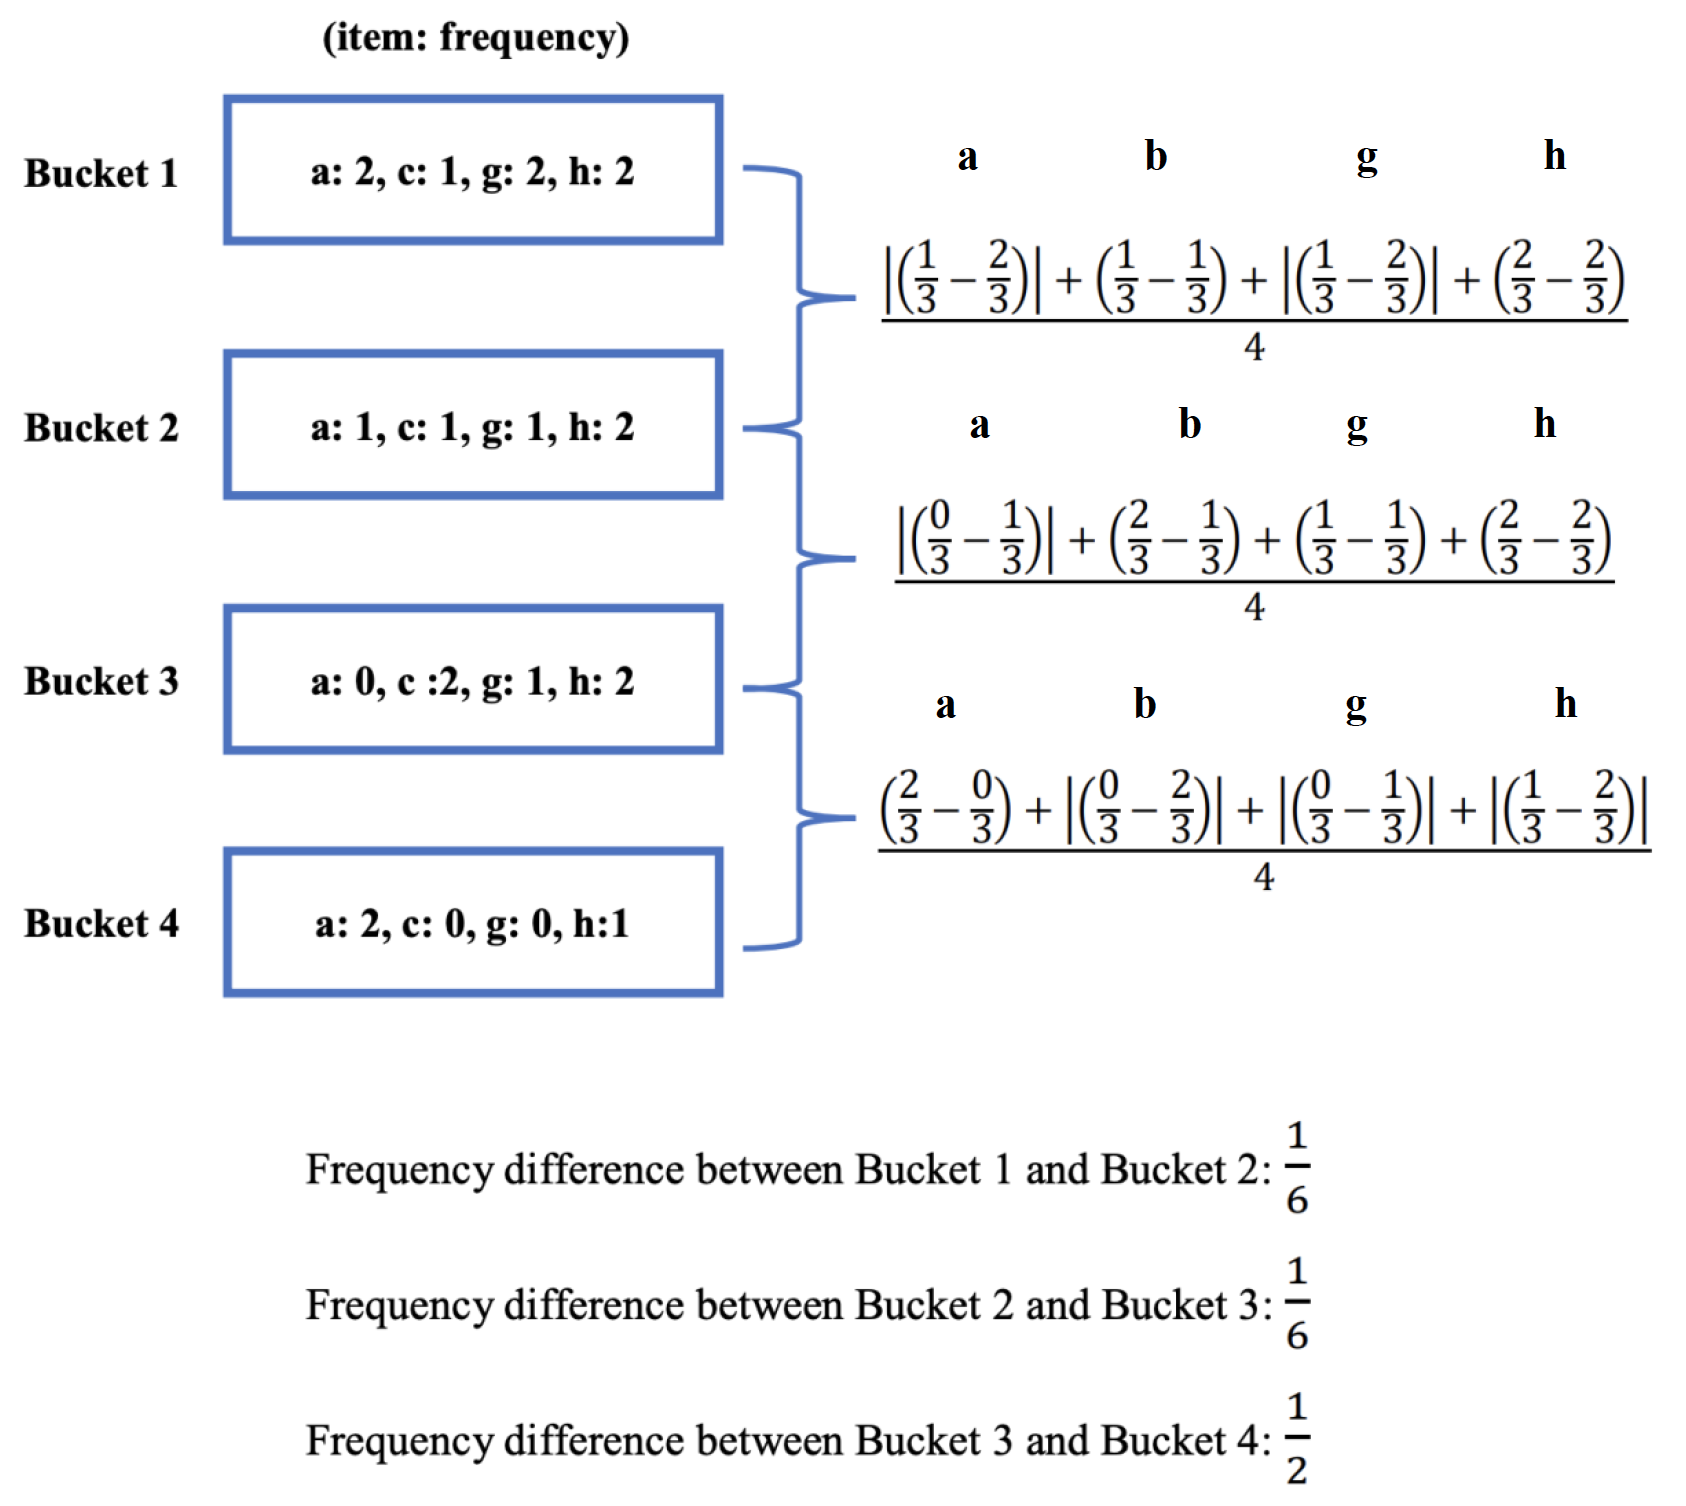
\includegraphics[scale=0.5]{Methodology/bsc.png}
\end{figure}

\section{Self-Sufficient Itemset Generation}
%What does this generator do?
We adapted the OPUS Miner proposed by Webb \cite{ssi}, for a dynamic streaming data. For a user-specified $k$ ($k=100$ by default) and interest measure, OPUS Miner find the top-$k$ productive non-redundant itemsets (as known as self-sufficient itemsets).

The original algorithm establishes a queue of items ordered in descending order on the upper bound on the value of any itemset that can include the item. However, one particular constraint with data stream algorithms is that there is only a one or limited pass through the data stream capability. This means the ability to run through an re-order of information is limited. In our self-sufficient Itemset Generator technique, we used the frequency counts from BSC to order the items instead. 
%Why we use this?

BSC provides an approximation of frequency counts for items, which helps us replace the static counting algorithm used in the original SSIG. The mining of the itemsets remains unmodified from the original version. 

%How does it work?

Our Self-Sufficient Itemset Generator algorithm is shown in Algorithm \ref{alg:ssig}.

\begin{algorithm}[h!]
\caption{Self-Sufficient Itemset Generator (SSIG)} 
\label{alg:ssig}
\hspace*{0.02in} {\bf Input:} 
$k$, \textit{frequentItems};\\
\hspace*{0.02in} {\bf Output:} 
\textit{result}($S$: set of self-sufficient itemsets);
\begin{algorithmic}[1]
\State OPUSMiner($k$, \textit{frequentItems})
\State $S \leftarrow$ result from OPUSMiner($k$, \textit{frequentItems})

\State \Return $S$: set of self-sufficient itemsets
\end{algorithmic}
\end{algorithm}


SSIG uses the list of frequent items obtain from BSC. We check for their interestingness and start to expand them into potential self-sufficient itemsets. Each newly generated itemsets and their partitions will be passed into SSIG to check for productivity and non-redundancy. Finally, all itemsets that passes the aforementioned constraints are considered as self-sufficient itemsets, $S$.

\begin{table}[H]
\caption{Set of 18 Transactions for SSIG}
\label{tb:tidlong}
\centering
 \begin{tabular}{p{4cm} p{4cm} p{4cm}}
 \hline\hline
 \multicolumn{3}{c}{Transactions (tid: items)}\\
 \hline
 1: a, g, h & 7: g & 13: a, c, h\\ 
 %\hline
 2: a, g, h, i & 8: c, h & 14: e, f, g\\
 %\hline
 3: b, c, d, f & 9: c, d, h & 15: a, b, e, h\\
 %\hline
 4: b, d, j & 10: b, f & 16: d, e, h\\
 %\hline
 5: c, f, h & 11: a, h & 17: a, e, g\\
 %\hline
 6: a, e, g, h & 12: a & 18: a, d, e, h\\
 \hline
\end{tabular}
\end{table}

\paragraph{An Example of SSIG}

Use the given dataset above in Table \ref{tb:tid}, we extended 6 more transactions for better mining result: Table \ref{tb:tidlong}. In this example, we will feed the following 18 transactions to SSIG to mine self-sufficient itemsets.

The mined self-sufficient itemsets from are $\{a, e\}, \{c, h\}$, and $\{e, h\}$.


\section{Regional Concept Drift Adaption}
%What does the RCDA do?
To retrieve non-drifted information from suspended historical data, similar to the buffer system \cite{buffer} used to find the best drift time point to identify concepts, we proposed a simple solution to identify regional drifts and integrate it into our self-sufficient itemset mining process.

The Regional Concept Drift Adaptor (RCDA) plays a key role in our ASSIM framework. It detects regional concept drifts in the generated self-sufficient itemsets. It analyses concept drifts and make decisions on where and when to re-mine additional items using SSIG.

%Why we have RCDA?
%Concept drifts can cause inaccurate mining result, for instance, the distribution of the existing self-sufficient itemsets changed, which means the data before the drift point cannot be used along with the data beyond that point. 
%How does it work?
%\subsubsection{ADaptive WINdowling (ADWIN)\cite{adwin}}
%The algorithm will decide the size of the window by cutting the statistics' window at different points and analysing the average of some statistic over these two windows. If the absolute value of the difference between the two averages surpasses a pre-defined threshold, change is detected at that point and all data before that time is discarded.
RCDA uses a well known drift detector, ADWIN \cite{adwin}, to detect concept drifts in the data streams. ADWIN monitors the changes in distribution between two windows, specifically, the distribution of the support of the self-sufficient itemsets found after the previous drift point, and the updated distribution of the supports that represents the current distribution. If there is a significant difference between the two windows a change is signalled. 

The na\"ive way to adapt to concept drifts is to re-mine the itemsets each time a drift has been detected, discarding all the old itemsets. This is inefficient as we may have lost valuable itemset information that may still be current. 

Our Regional Concept Drift Adaptor algorithm is shown in Algorithm \ref{alg:rcda}.

\begin{algorithm}[h!]
\caption{Regional Concept Drift Adaptor (RCDA)} 
\label{alg:rcda}
\hspace*{0.02in} {\bf Input:} 
data stream $\mathcal{D}$, a set self-sufficient itemsets $S$;\\
\hspace*{0.02in} {\bf Output:} 
\textit{Updated set of self-sufficient itemsets $S$};
\begin{algorithmic}[1]

\State Initialise window $\mathcal{W}$ for ADWIN and empty buffer $\mathcal{B}$
%\State Boolean: $hasChange \leftarrow $FALSE

\For{each self-sufficient itemset $s$ in $S$} 
  \State ADWIN($s$, $\mathcal{D}$)
  \If{drift detected} 
    \State $i \leftarrow$ number of TID when drift detected
    \If{$s\in \{T_1, T_2, ..., T_i\}$}
        \State update $sup(s)$
    \Else
        \State $\mathcal{B} \leftarrow T_i$
    \EndIf
    \State ADWIN($s$, $\{T_i, ..., T_n\}$)
    \If{next drift signalled}
        \State $S' \leftarrow$ SSIG($\mathcal{B}$)
    \EndIf
  \EndIf
\EndFor

\State Append new self-sufficient itemsets $S'$ to $S$: $S = S + S'$

\State \Return set of updated self-sufficient itemsets
\end{algorithmic}
\end{algorithm}

RCDA is designed to overcome this problem by storing previously mined self-sufficient itemsets along with its frequency. The approach works as follows.
Each itemset is monitored using its own drift detector. As a transaction, $T$, in the data stream appears we check whether it contains any of the self-sufficient itemsets $S$, whereby $\exists S \in T$. If the itemsets exists, we will update the support of the itemsets. If none of the itemsets in $S$ exist in $T$ then we store the transaction in a buffer, $B$. We re-mine $B$ using SSIG when the next drift point is signaled.  

The intuition is that transactions that do not contain pre-existing itemsets may contain new knowledge on the data. Thus, by capturing and re-mining that portion of the stream, we are essentially looking for new itemsets that are just appearing in the new incoming data stream. This region of data do not contain any previously found itemsets would not be considered from the same distribution.

We also remove any itemsets that are no longer found in the current data stream. For example we may have an self-sufficient itemset $A$ that has appeared in the data stream previously but the support of this itemset has drop significant in the current time window measured from the previous drift point to current point, and no longer satisfy the thresholds.  

\paragraph{An Example of RCDA}

Use the given dataset above in Table \ref{tb:tidlong}. In this example, we will perform regional drift detection on two self-sufficient itemsets mined from SSIG: $\{a, h\}$ and $\{e, h\}$.

\begin{table}[H]
\caption{Set of 18 Transactions for RCDA}
\label{tb:tidlong1}
\centering
 \begin{tabular}{p{4cm} p{4cm} p{4cm}} 
 \hline\hline
 \multicolumn{3}{c}{Transactions (tid: items)}\\
 \hline
 1: a, g, h & 7: g & 13: a, c, h\\ 
 %\hline
 2: a, g, h, i & 8: c, h & 14: e, f, g\\
 %\hline
 3: b, c, d, f & 9: c, d, h & 15: a, b, e, h\\
 %\hline
 4: b, d, j & 10: b, f & 16: d, e, h\\
 %\hline
 5: c, f, h & 11: a, h & 17: a, e, g\\
 %\hline
 6: a, e, g, h & 12: a & 18: a, d, e, h\\
 \hline
\end{tabular}
\end{table}

Our drift detectors use occurrences of self-sufficient itemset in each transaction as input, which is either TRUE (1) or FALSE (0). The input and result of $\{a, h\}$ and $\{e, h\}$ will be shown in Table \ref{tb:ah} and Table \ref{tb:eh}.

\begin{table}[H]
\caption{RCDA Detects Drifts for $\{a, h\}$}
\label{tb:ah}
\centering
 \begin{tabular}{p{4cm} p{4cm} p{4cm}} 
 \hline\hline
 \multicolumn{3}{c}{Transactions (tid: occurrence of $\{a, h\}$)}\\
 \hline
 1: 1 & 7: 0 $\leftarrow drift$ & 13: 1\\ 
 %\hline
 2: 1 & 8: 0 & 14: 0\\
 %\hline
 3: 0 & 9: 0 & 15: 1\\
 %\hline
 4: 0 & 10: 0 & 16: 0\\
 %\hline
 5: 0 & 11: 1 $\leftarrow drift$ & 17: 0\\
 %\hline
 6: 1 & 12: 0 & 18: 1\\
 \hline
\end{tabular}
\end{table}

Table \ref{tb:ah} gives the first drift point which is at TID 7, which will trigger RCDA to check for $\{a, h\}$'s occurrence before TID 7. In this case, $\{a, h\}$ exists in TID 1, 2 and 6, so we update the support of $\{a, h\}$ to 3 and keep running RCDA on the rest of the data stream.

\begin{table}[H]
\caption{RCDA Detects Drifts for $\{e, h\}$}
\label{tb:eh}
\centering
 \begin{tabular}{p{4cm} p{4cm} p{4cm}} 
 \hline\hline
 \multicolumn{3}{c}{Transactions (tid: occurrence of $\{e, h\}$)}\\
 \hline
 1: 0 & 7: 0 & 13: 0\\ 
 %\hline
 2: 0 & 8: 0 & 14: 0\\
 %\hline
 3: 0 & 9: 0 & 15: 1 $\leftarrow drift$ \\
 %\hline
 4: 0 & 10: 0 & 16: 1\\
 %\hline
 5: 0 & 11: 0 & 17: 0\\
 %\hline
 6: 1 $\leftarrow drift$ & 12: 0 & 18: 0\\
 \hline
\end{tabular}
\end{table}

Table \ref{tb:eh} above detects the first drift point at TID \#6. When RCDA starts to look at the occurrence of $\{e, h\}$ before TID \#6, it comes out zero. In this case, we store this transaction TID \#$6: a, e, g, h$ in a buffer $\mathcal{B}$ and wait for the next drift signal. At TID \#15, RCDA is triggered to start SSIG to remine the buffer $\mathcal{B}$. The result will be appended into the old set of self-sufficient itemsets mined by SSIG.

\section{Sliding-window Model}

The methods that incrementally mine association rules in dynamic databases have been widely discussed \cite{SWF,window,inc}. In these methods, all the frequent itemsets and their support counts derived from the original database are retained. When transactions are added or expired, the support counts of the frequent itemsets contained in
them are recomputed. By reusing the frequent itemsets and their support counts retained, the number of candidate itemsets generated during the mining process can be reduced. All these methods have to re-scan the original database because non-frequent itemsets can be
frequent after the database is updated. Therefore, they cannot work without seeing the entire database and cannot be applied to data streams.  

To make ASSIM work on an actual online mode, we propose a sliding-window model to solve the problem of incremental mining of self-sufficient itemsets in data streams. 

\subsection{Sliding-window Miner (SM)}

Our sliding-window miner uses a time-sensitive sliding-window model to solve data stream mining problem in a online mode which was proposed by Chen et al. \cite{timewin}.

\subsubsection{Time-sensitive Sliding-window (TS)}

Given a time point $t$ and a time period $p$, the set of all the transactions arriving in $[t-p+1, t]$ will form a basic block. A transactional data stream is decomposed into a sequence of basic blocks of transactions, which are assigned with serial numbers starting at 1. Given a window with length $|W|$, we slide it over this sequence to see a set of overlapping sequences, where each sequence is called the time-sensitive sliding-window TS.

Let the basic block numbered $i$ be denoted as $B_i$. The number of transactions in $B_i$ is denoted as $|B_i|$, which is not fixed due to the variable data arrival rate. For each $B_i$, the TS that consists of the $|W|$ consecutive basic blocks from $B_i_-_|_W_|_+_1$ to $B_i$ is denoted as $TS_i$. %Let the number of transactions in $TS_i$ be denoted as $\Sigma i$. 

\subsubsection{Self-Sufficient Itemsets in $TS_i$} 

An itemset $x$ is self-sufficient in $TS_i(B_i)$ if $x$ is productive, non-redundant and independently productive, $x$ needs to satisfy the following conditions:

\begin{enumerate}
    \item Every subset $y$ of $x$: $y\subset x$ is associated with its complementary set: $x\setminus y$.
    \item $x$ contains no subset $z$: $z\subset x$, that contains an item $i$, that subsumes $z\subset i$.
    \item The productivity of $x$ cannot be explained by the productivity of its self-sufficient supersets.
\end{enumerate}

Owing to the characteristics of data streams, it is not realistic to scan the past basic blocks recursively for mining self-sufficient itemsets in each of the subsequent TS. In this section, we assume that only the summary information derived from $TS_i-1$ is provided for mining self-sufficient itemsets in $TS_i$. We use a scenario to illustrate the mining process in Figure \ref{fig:fsl}, where the basic unit is transactions in the first hour and $|W|$ is 4. As the new basic block $B_4$ comes, the oldest basic block $B_1$ in $TS_1$ is expired. To find self-sufficient itemsets in $TS_2$, we consider three kinds of itemsets from two sources, the self-sufficient itemsets in $TS_1$ and the self-sufficient ones in $B_5$, as follows:

\begin{enumerate}
\item An itemset which is self-sufficient in $TS_1$ still remains self-sufficient in $TS_2$ after $B_5$ appended.
\item Appended data stream $B_5$ brings new self-sufficient itemsets.
\item An itemset which is not self-sufficient in $TS_1$ becomes self-sufficient in $TS_2$.
\end{enumerate} 

By utilising the definition of self-sufficient and the constraint of productivity and non-redundancy, the following lemmas are generally used in Sliding-window Miner (SM).

\begin{lemma}
An itemset which is self-sufficient in $TS_1$ will still remains self-sufficient in $TS_2$.
\end{lemma}

\begin{proof}
According to the definition of self-sufficient itemset \cite{ssi}: if an itemset $x$ is self-sufficient, every $y\subset x$ will be associated with $x\setminus y$. After appending $B_5$, the old associations between subsets of mined self-sufficient itemsets still exist which make the existing self-sufficient itemsets remain true.
\end{proof}

$B_5$ may bring some new associations into the data stream, some itemsets determined not self-sufficient may become self-sufficient. New items also bring some potential self-sufficient itemsets consists with part of the new items.

\begin{figure}[H]
\caption{Time-sensitive sliding-window model}
\label{fig:fsl}
\centering
%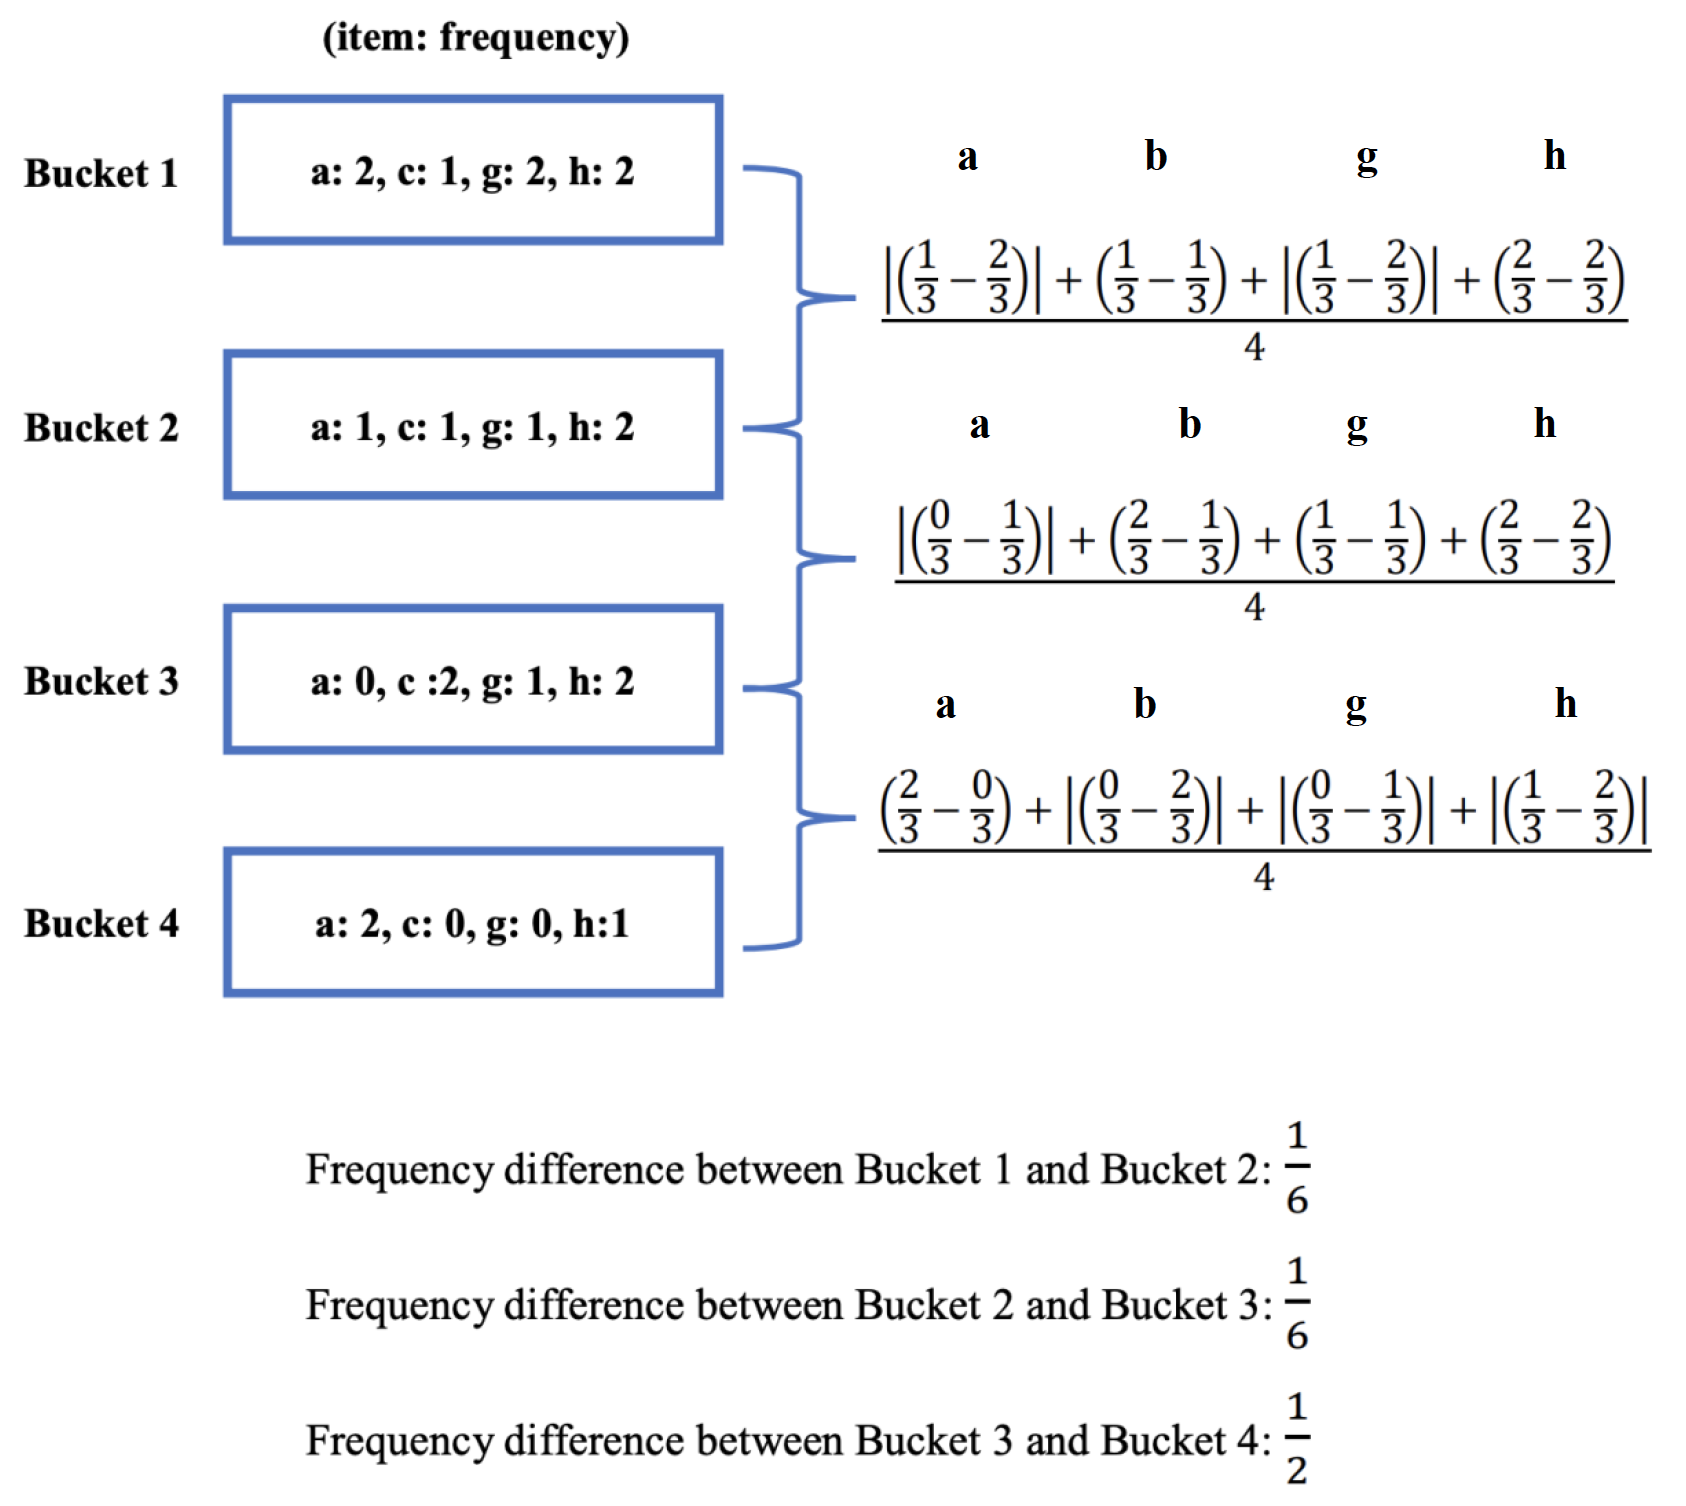
\includegraphics[width=\textwidth]{Methodology/bsc.png}
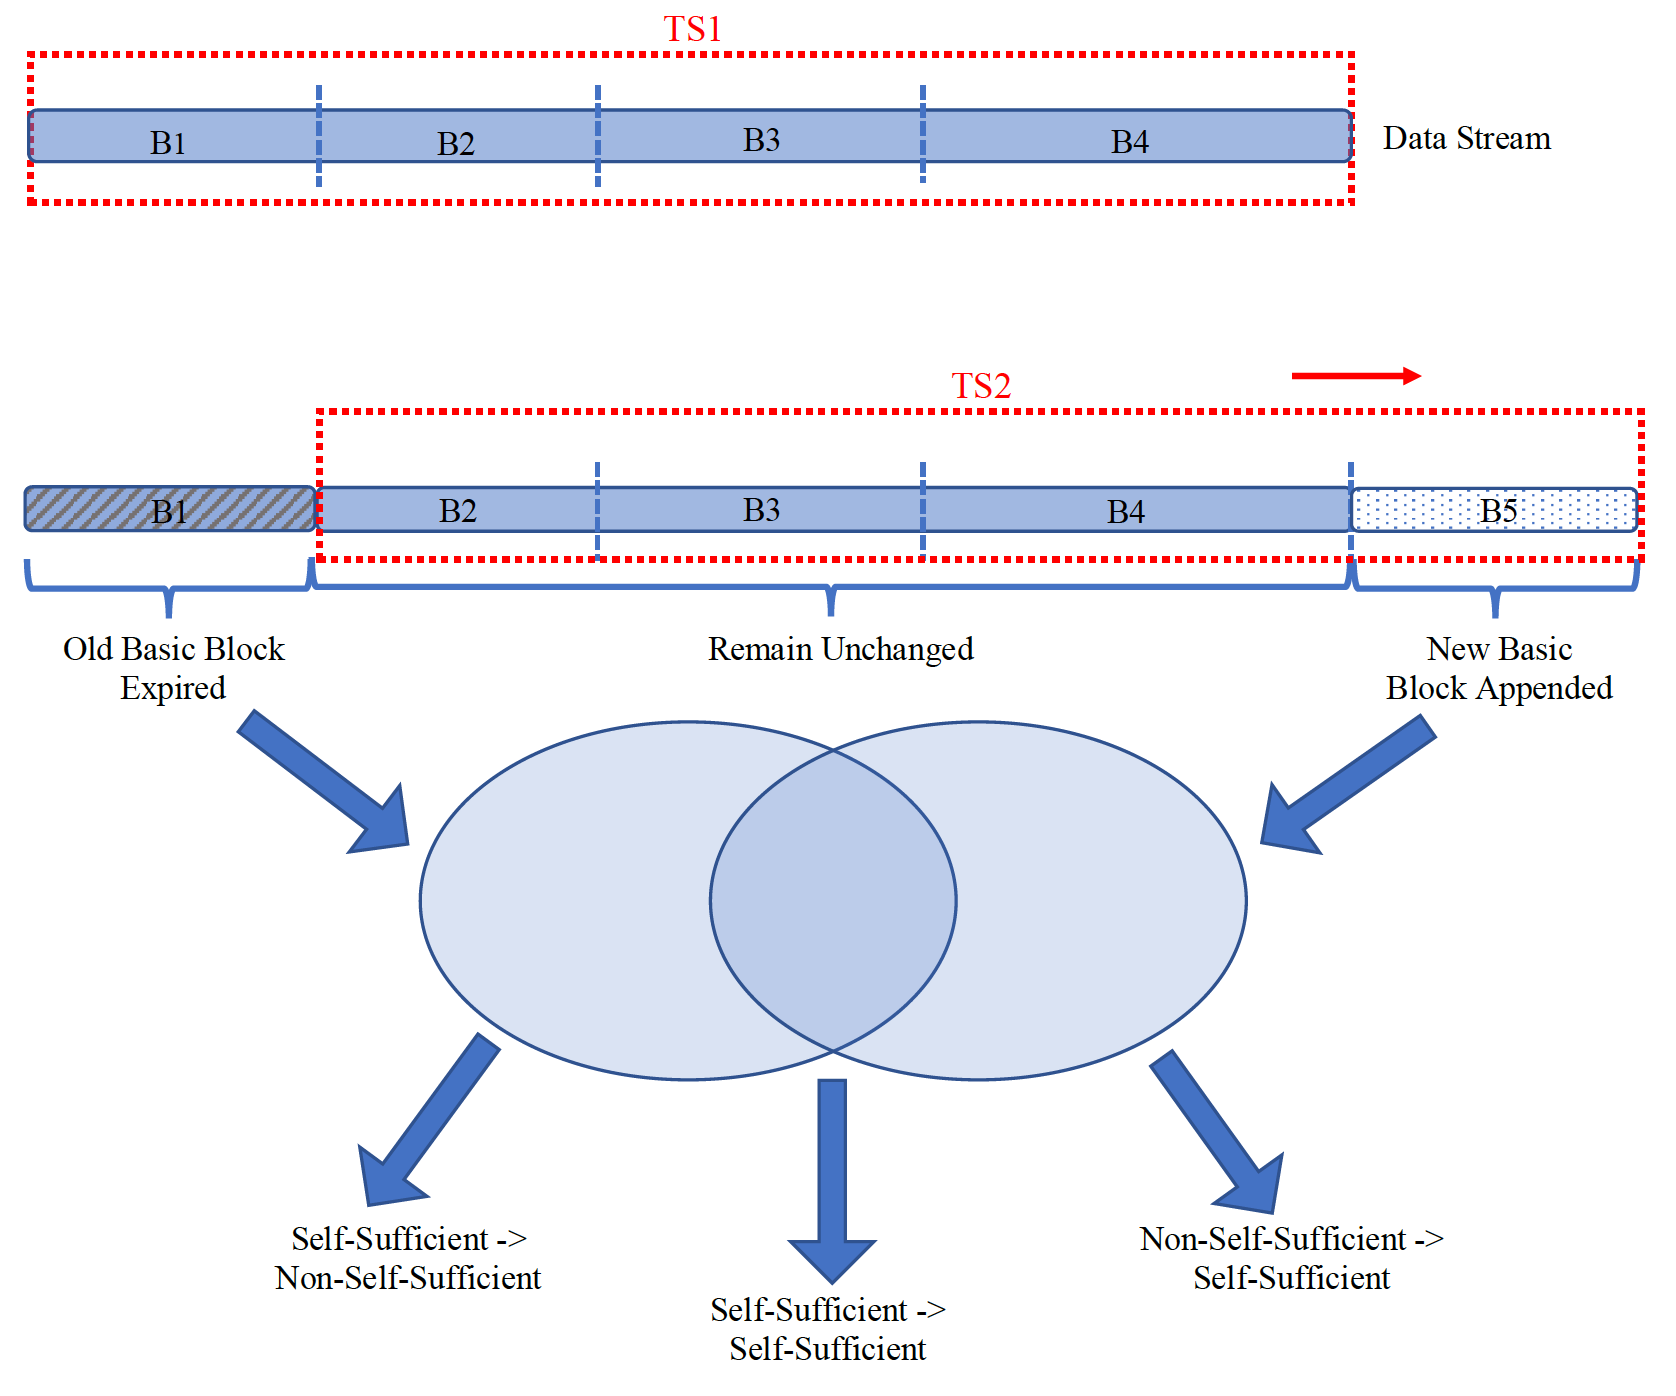
\includegraphics[scale=0.45]{Methodology/TSL.png}
\end{figure}

\subsection{Framework}
Instead of dividing data stream into batches prior to the mining process, Sliding-window Miner (SM) makes some adjustments to help SSIG work in an incremental data stream which achieves the actual real-time mining. 

Consider the two out of three kinds of self-sufficient itemsets mentioned above (the first one has been approved not applicable), we check the appended data stream $B_5$ for self-sufficient itemsets contains new-coming items first. This can be finished by running our SSIG on the appended data stream $B_5$ and store the results.

Next step is to mine itemsets which just turned self-sufficient after the update. These can be those itemsets whose subsets did not have enough associations with the remainder in the expired $B_1$ and remaining $B_2, B_3$. 

In this sliding-window method, we only use the frequency counter of BSC on $TS_1$ to generated a list of frequent items with their frequencies $F$. When $TS_1$ has been fed into SSIG to produce a set of self-sufficient itemsets $S$, the non-expanded items in $F$ will be separated into a new list $F'$. A data stream may be divided into blocks with different numbers of transactions. The buffer continuously consumes transactions and pours them block-by-block into our system. When a new basic block or even a single transaction produced, update $F'$ if it contains any item from $F'$ and feed $F'$ into SSIG to generate new self-sufficient itemsets. This process is illustrated in Fig \ref{fig:smframe}.

\begin{figure}[H]
\caption{How sliding-window miner processes new incoming data}
\label{fig:smframe}
\centering
%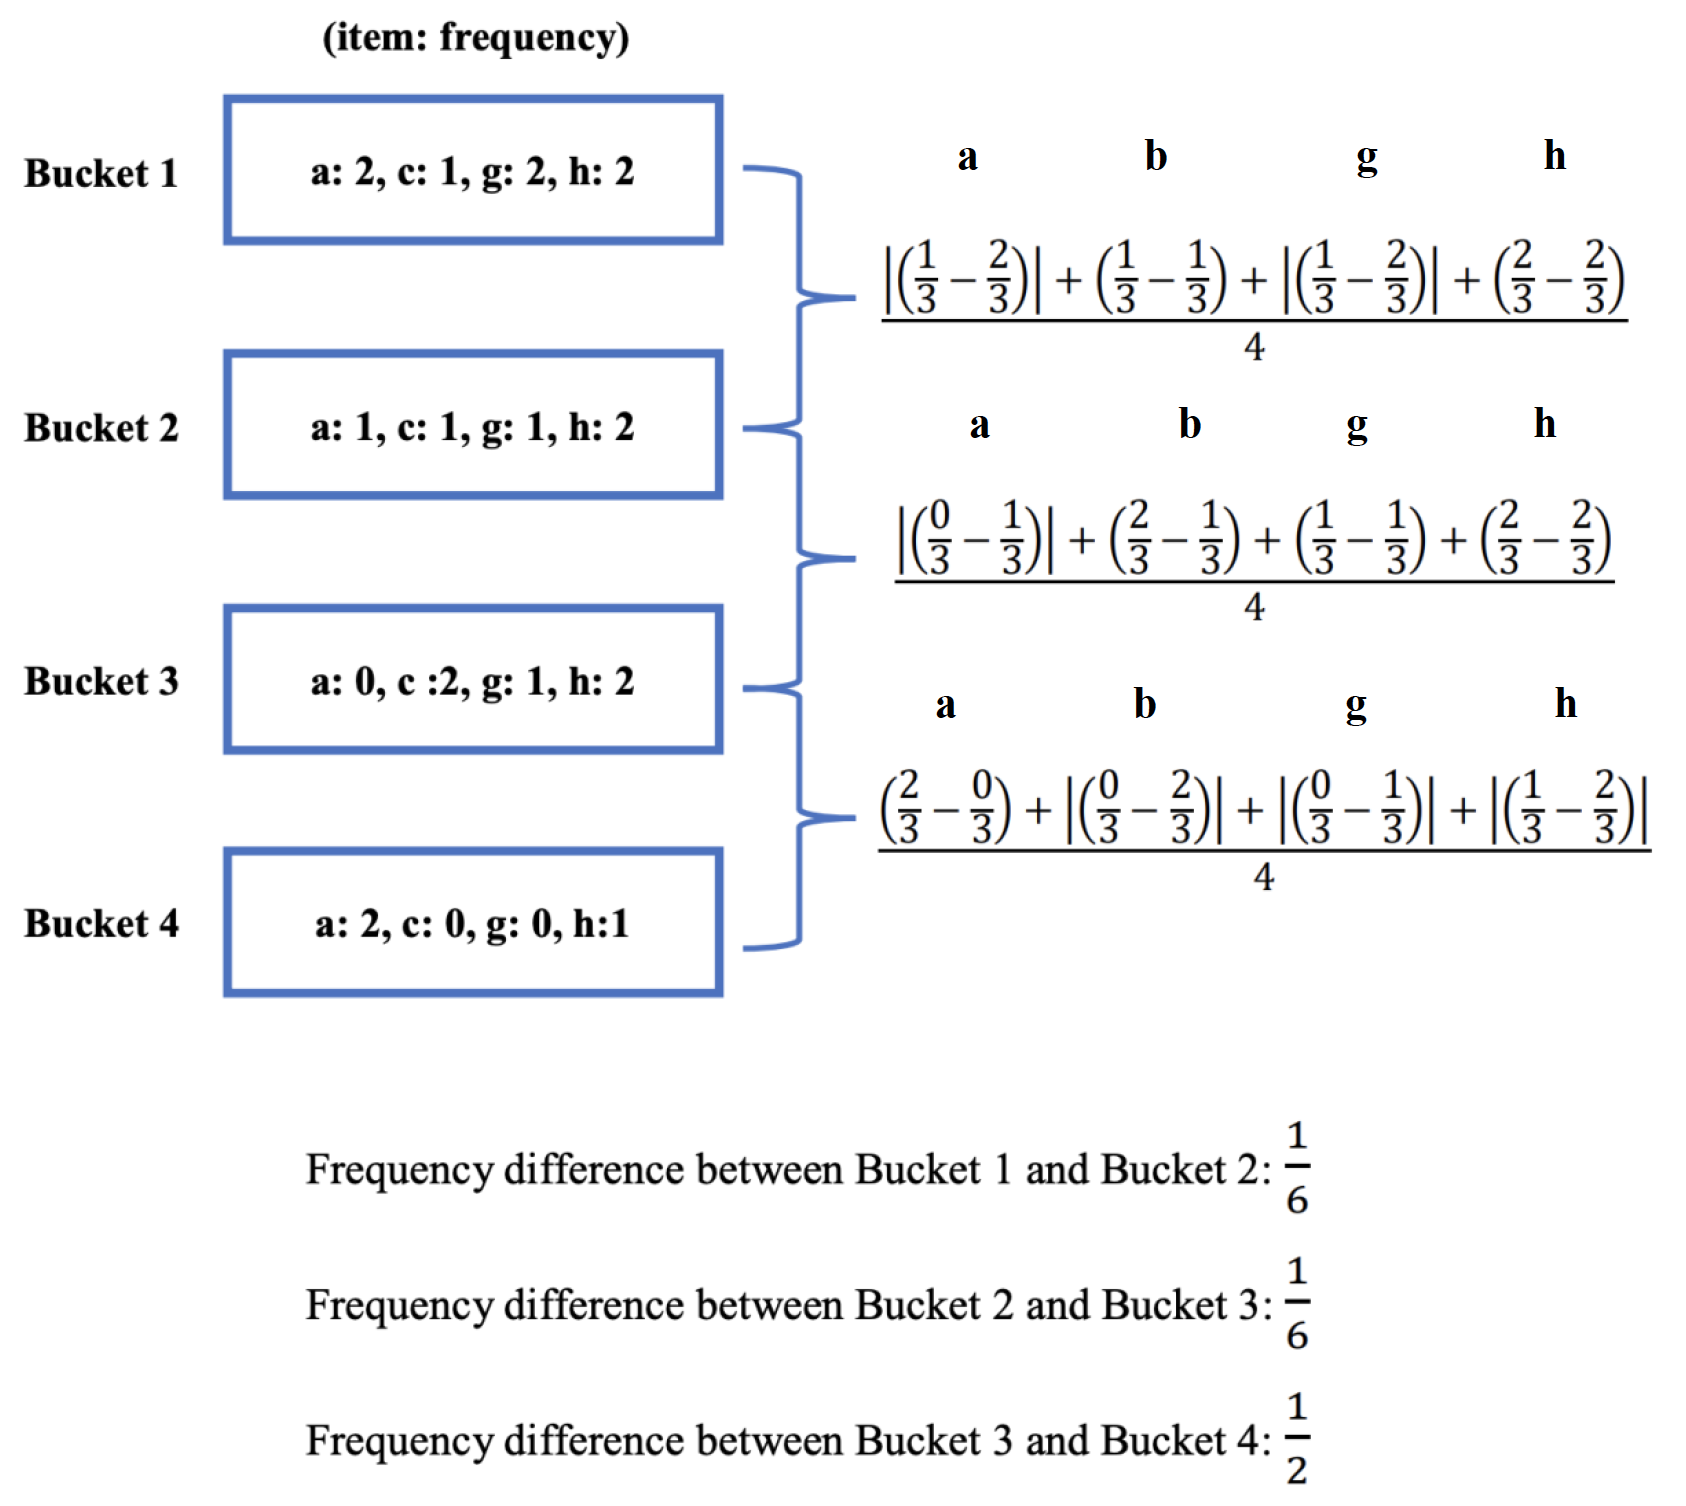
\includegraphics[width=\textwidth]{Methodology/bsc.png}
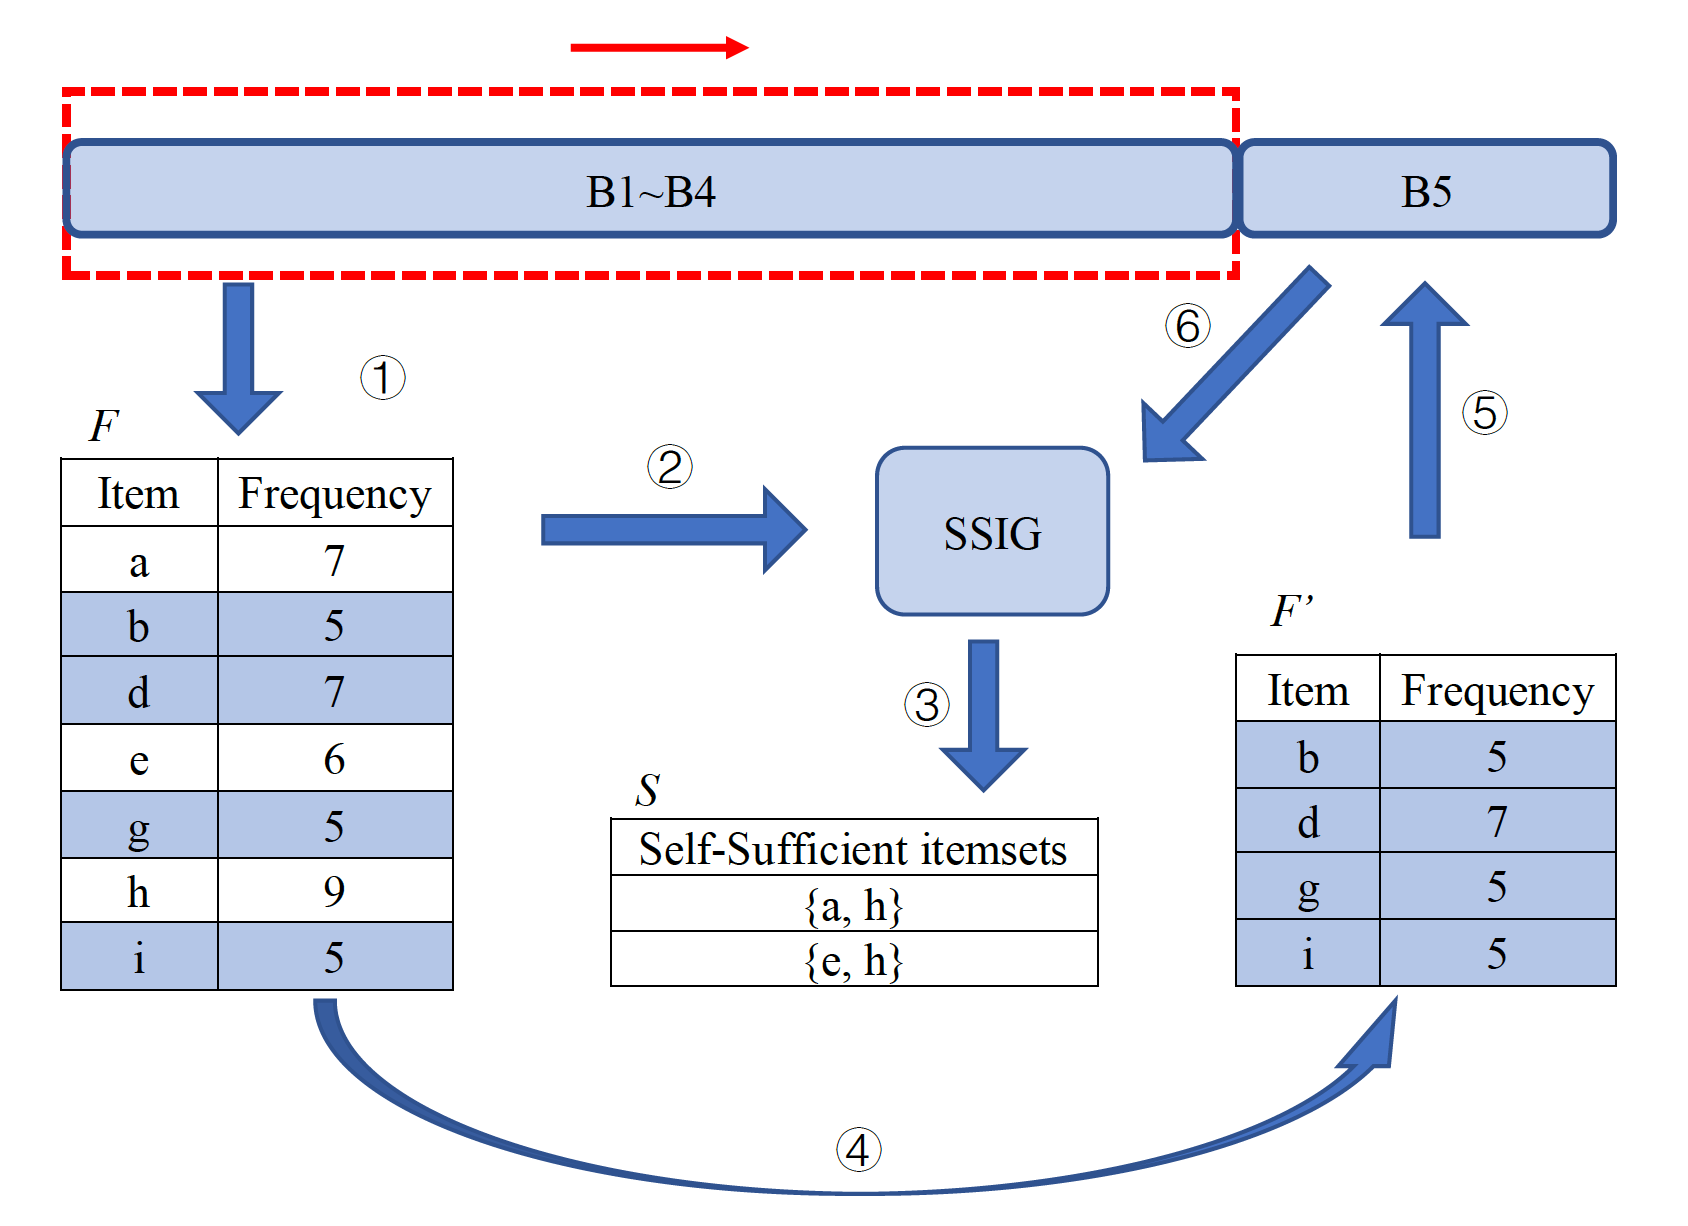
\includegraphics[scale=0.5]{Methodology/frame.png}
\end{figure}

\subsection{Discussion}
Sliding-window Miner has the ability to using a moving window to process data stream incrementally which make up the drawbacks of batch processing we proposed in ASSIM. Because of the limitation of time of this dissertation, we only discuss the Sliding-window Miner technique at the conceptual level. But it is worthy to be developed and experiment its efficiency and compatibility on actual online learning.

\section{Summary}

Interesting association discovery is often a more complicated and computationally expensive task than frequent itemset mining. Besides the traditional ``support-confidence'' framework for association rule mining, the definition of self-sufficient itemset changed the way of determining interestingness of association rules. It is defined as each of a self-sufficient itemset's subset must be associated to its complement. The original efficient self-sufficient miner, also as known as OPUSMiner, achieves an outstanding efficiency, also proved effective and accuracy. While OPUSMiner was developed on a static database, to satisfy the urgent need of data stream adaption, we remedy OPUSMiner by providing a stable batch calculator to produce stable batches and sketch frequent items. To minimise the error brings by underlying distribution changes, also as known as concept drifts in data streams, we added a concept drift adaptor which is able to detect and adapt to underlying drifts. Besides the fact that most mainstream concept drift detector discard data prior to the drift point, which usually miss the regional drift. Our Regional Concept Drift Adaptor provides regional drift detection and adaption for self-sufficient itemset mining. Using batch processing is not actual online learning in fact, we also discussed the sliding-winder miner, which uses a time-sensitive sliding window to mine self-sufficient itemsets from a data stream.

In the next chapter, we will perform several experiments to test the efficiency and effectiveness of our proposed framework.